\section{OpenFOAM}
\label{Kapitel:AnhangOpenFOAM}
Dieses Kapitel soll eine Übersicht über \openfoam{} und die darin eingebauten Computercodes geben.
Die Notation verwendet \fileemph{Kursivschrift} für Computer"-datei-Namen und \openfoam{}-spezifische Begriffe. Für für Computercodes wie Programme oder Teile davon wird \codeemph{Schreibmaschinenschrift} verwendet.

Ein Simulationslauf in \openfoam{} wird \fileemph{case} genannt, der durch ein Verzeichnis auf dem Computer repräsentiert wird. Da \openfoam{} keine gra\-phi\-sche Benutzeroberfläche besitzt, werden alle Informationen und Resultate in Textdateien gespeichert, die in diesem \fileemph{case} abgelegt werden.\\
Die Informationen sind aufgeteilt in die Unterverzeichnisse \fileemph{0}, \fileemph{constant} und \fileemph{system}, sowie Zeitschrittverzeichnisse die nach der jeweiligen Zeit benannt sind. Abbildung~\ref{fig:ofCaseSchema} zeigt die schematische Darstellung.\\ %In den darin gespeicherten Dateien stehen alle Informationen über die Simulation und deren Resultate.\\
Im Verzeichnis \fileemph{0} sind die Anfangs- und Randbedingungen der Simulation definiert. Die darin enthaltenen Dateien sind nach den entsprechenden Variablen genannt wie z.B. \fileemph{p} für den Druck oder \fileemph{U} für die Geschwindigkeit.
In \fileemph{constant} stehen die Simulationsparameter wie zum Beispiel das verwendete Viskositätsmodell und dessen Parameter. Ausserdem ist im Unterverzeichnis \fileemph{polymesh} die Geometrie definiert.
In \fileemph{system} sind schliesslich die Simulationskontrollgrössen enthalten. Dazu gehören in der Datei \fileemph{controlDict} die Anzahl der Zeitschritte und deren Länge, in \fileemph{fvSchemes} die verwendeten Diskretisierungsschemen und in \fileemph{fvSolution} welche Lösungsmethoden für die linearen Gleichungssystem verwendet werden.

\begin{figure}
    \centering
    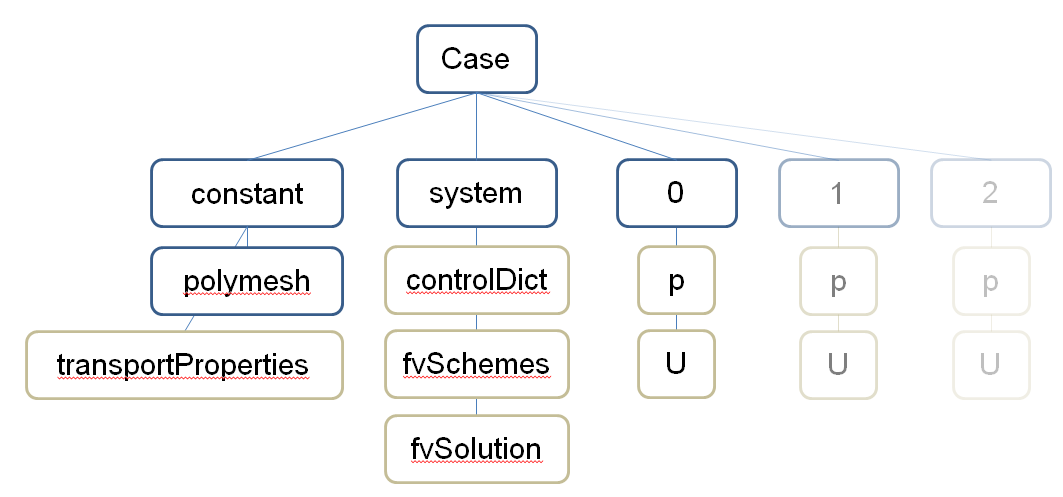
\includegraphics[width=\textwidth]{figures/OfCaseSchema.png}
    \caption{Der schematische Aufbau eines \openfoam{} 'cases'. Die blauen Einträge sind Verzeichnisse, die braunen stellen Dateien dar.}
    \label{fig:ofCaseSchema}
\end{figure}
%
\subsection{Löser}
Ein Löser in \openfoam{} ist ein \cpp{} Programm, das in einem \fileemph{case} arbeitet. Der Löser ruft dabei die Informationen aus den im \fileemph{case} enthaltenen Verzeichnissen ab und benützt diese, um einen Simulationslauf zu definieren. Danach beginnt er die Simulation und erzeugt neue Zeitschritt-Verzeichnisse, in denen er den berechneten Zustand des Systems zu einem späteren Zeitpunkt abspeichert.

\subsubsection{simpleFoam}
Für die scherratenabhängigen Viskositätsmodelle wurde als Basislöser die schon in \openfoam{} eingebaute Version \codeemph{simpleFoam} des SIMPLE Algorithmus verwendet.
Diese erlaubt es unter verschiedenen schon implementierten Viskositätsmodellen zu wählen, oder diese zu modifizieren um ein eigenes Modell zu implementieren.\\
Dabei wird in der Datei \fileemph{transportProperties} als Transportmodell das gewünschte konstitutive Modell mit seinen Parametern hinterlegt:
%
\subsubsection{timeAdjustNonNewtIcoFoam}
Der Löser zu der in \openfoam{} implementierten Version des PISO Algorithmus heisst \codeemph{icoFoam}.
Diese Version unterstützt aber keine nicht-Newtonsche Modelle und ist nicht in der Lage, den Zeitschritt an die maximal auftretende Geschwindigkeit anzupassen.\\
Um trotzdem in der Lage zu sein nicht-Newtonsche, transiente Probleme zu lösen, wurde im Rahmen dieser Arbeit der Löser \codeemph{icoFoam} erweitert.

Analog zum Löser \codeemph{simpleFoam} wird zu Beginn der Simulation eine Instanz der Klasse \codeemph{transportModel} initialisiert, die dann in jedem Zeitschritt die kinematische Viskosität aktualisiert und zur Verfügung stellt:
%
\begin{lstlisting}
...
singlePhaseTransportModel fluid(U, phi);
...
while (runTime.run()) {
fluid.correct();
nu_ = fluid.nu();
}
...
\end{lstlisting}
%
Zusätzlich wurde in der Zeitschleife die von \openfoam{} zur Verfügung gestellte Routine \codeemph{setDeltaT.H} eingefügt, um $\Delta t$ in jedem Zeitschritt zu überprüfen und gegebenenfalls anzupassen.\\
Mit dieser Änderung können im \fileemph{controlDict} die Zeilen
%
\begin{lstlisting}
adjustTimeStep yes;
maxCo 0.5;
maxDeltaT 1;
\end{lstlisting}
%
eingefügt werden, um den Zeitschritt variabel zu machen.

Der resultierende Code \codeemph{timeAdjustNonNewtIcoFoam} ist in der Lage, sowohl mit nicht konstanten Viskositäten zu rechnen, als auch den Zeitschritt so zu wählen dass eine vom Nutzer bestimmte Courant Zahl nicht überschritten wird.\\
Die Courant oder auch CFL Zahl ist dabei definiert als Verhältnis zwischen Zeitschritt und räumlicher Auflösung und ist massgeblich für die Stabilität der Simulation
%
\begin{equation}
    c := \frac{\u\cdot \Delta t}{\Delta x} \overset{!}{<} 1.
\end{equation}
%
\subsubsection{viscoelasticFluidFoam}
Der Löser für die viskoelastischen Simulationen wurde von J.~Favero implementiert. Der Code ist eine Implementation des DEVSS Algorithmus, der aber für die Berechnung der Schubspannungsterme auf eine separat implementierte Klasse zurückgreift.\\
Dieser Code wurde unverändert übernommen und ist hier nur der Komplettheit halber aufgeführt.
%
\subsection{Rheologische Modelle}
Die rheologischen Modelle können in \openfoam{} als Bibliotheken eingebaut werden. Dazu wird ihr Code kompiliert und im \fileemph{controlDict} angegeben, welche Bibliotheken verwendet werden sollen. Sie sind keine eigenständigen Programme, sondern werden von den Lösern benutzt um Teile der Berechnung auszuführen.
%
\subsubsection{Scherratenabhängige Modelle}
Die Implementation eigener Modelle wurde realisiert indem eine neue \cpp{} Klasse implementiert wurde, die von der in \openfoam{} vorhandenen Klasse \codeemph{viscosityModel} abgeleitet ist.
Diese neue Klasse muss die Funktionen \codeemph{nu} und \codeemph{correct} zur Verfügung stellen. \codeemph{nu} gibt die die kinematische Viskosität zurück, \codeemph{correct} berechnet diese neu.
Dabei kann durch die von der Basisklasse zur Verfügung gestellte Funktion \codeemph{strainRate} auf die Scherrate $\gammap$ zurückgegriffen werden. Das Einlesen von zusätzlichen Parametern geschieht dabei in der Funktion \codeemph{read}.

Der schematische Aufbau solch einer Klasse:
%
\begin{lstlisting}
class limitedHerschelBulkley : public viscosityModel {
    tmp<volScalarField> nu() const {
        return nu_;
    }
    void correct() {
        nu_ = calcNu();
    }
    bool read(const dictionary& viscosityProperties) {
        ...
    }
};
\end{lstlisting}
%
In der Funktion \codeemph{correct} wird hier eine private Funktion \codeemph{calcNu} aufgerufen, die die Viskosität neu berechnet.
Das modifizierte Herschel-Bulkley Modell \eqref{eq:modHB} kann dabei, dank der sehr mächtigen Operatorüberladung von \openfoam{}, in einer sehr kompakten Schreibweise implementiert werden:
%
\begin{lstlisting}
Foam::tmp<Foam::volScalarField>
calcNu() {    
    return
    (
     min(
         nu0_,
         ( tau0_ * (1.001-exp(-1*m_*sr()))  + k_ *rtone* pow( tone*sr(),n_ ) )
         /(max(sr(), dimensionedScalar ("VSMALL", dimless/dimTime, VSMALL)))
        )
    );
}
\end{lstlisting}
%
wobei \codeemph{sr()} die Scherrate ist und \codeemph{tau0\_}, \codeemph{k\_} und \codeemph{n\_} die Modellparameter sind.\\
Durch die Division durch das Maximum der Scherrate und \codeemph{VSMALL}, einer sehr kleinen Konstante, wird die Division durch Null vermieden.\\
Da das Herschel-Bulkley Modell eine unendliche Viskosität vorsieht wenn das Fluide nicht geschert wird, dies aber zu numerischen Problem führen kann, wird ausserdem die Viskosität nach oben hin durch die Nullviskosität \codeemph{nu0\_} beschränkt.
%
\subsubsection{Viskoelastische Modelle}
Der Löser \codeemph{viscoelasticFluidFoam} greift für die Berechnung des Schubspannungtensors auf eine separate Klasse \codeemph{viscoelasticModel} zurück, die ähnlich der \codeemph{transportModel} Klasse in \codeemph{simpleFoam} die Methoden \codeemph{divTau} und \codeemph{correct} zur Verfügung stellt.\\
Die Methode \codeemph{divTau} berechnet dabei die Divergenz der Schubspannung $\T$ und implementiert gleichzeitig noch einen Teil der DEVSS Methodik indem sie die Split Stress Terme dazu addiert:
%
\begin{lstlisting}
Foam::tmp<Foam::fvVectorMatrix>
divTau(volVectorField& U) const {
    ...
    return
    (
        fvc::div(tau_/rho_, "div(tau)")
      - fvc::laplacian(etaPEff/rho_, U, "laplacian(etaPEff,U)")
      + fvm::laplacian( (etaPEff + etaS_)/rho_, U, "laplacian(etaPEff+etaS,U)")
    );
}
\end{lstlisting}

In der Methode \codeemph{correct} wird bestimmt, wie sich der Schubspannungstensor von einem Zeitschritt zum nächsten ändert.\\
Diese Methode ist der Teil der Klasse, der an das gewünschte viskoelastische Modell angepasst werden muss. Das in dieser Arbeit verwendete White-Metzner Modell \eqref{eq:whiteMetznerModell} benötigt für das Update des Schubspannungstensors drei Schritte.
In einem ersten Schritt müssen die direkt von $\u$ abhängigen Variablen berechnet werden
\begin{lstlisting}
volTensorField L = fvc::grad(U());
volTensorField C = tau_ & L;
volSymmTensorField twoD = twoSymm(L);
volScalarField gamma = sqrt(2.0) * mag(symm(L));
\end{lstlisting}

In einem zweiten Schritt werden die scherratenabhängige Relaxationszeit $\lambda$ und Viskosität $\eta$ aktualisiert
\begin{lstlisting}
volScalarField etaPValue =
     max(
         etaMin_,
         min(
             etaMax_,
             ( tau0_ + K_ * rtone * Foam::pow( tone*gamma,n_ ) )
             /(max(gamma, dimensionedScalar ("VSMALL", dimless/dimTime, VSMALL)))
         )
     );

volScalarField lambdaValue = 
        lambdaInf_+(lambdaNull_-lambdaInf_) * 
                Foam::pow(
                1 + Foam::pow( L_* gamma,b_), 
                (nLambda_- 1)/b_
                );
\end{lstlisting}
%
Als letztes wird die Differentialgleichung mit dem Transport-Term implizit gelöst
%
\begin{lstlisting}
fvSymmTensorMatrix tauEqn
(
    fvm::ddt(tau_)
    + fvm::div(phi(), tau_)
    ==
    etaPValue/lambdaValue*twoD
    + twoSymm(C)
    - fvm::Sp(1/lambdaValue, tau_)
);
           
tauEqn.relax();
tauEqn.solve();
\end{lstlisting}
%
\subsection{Nachbearbeitung}
Für die Auswertung der Simulationen gibt es mit ParaView \cite{paraview} und diversen \openfoam{} Utilities schon eine ganze Anzahl von Möglichkeiten.\\
In dieser Arbeit wurde zusätzlich noch die Möglichkeit genutzt eigene Runtime Functions zu schreiben, also Funktionen die schon während der Simulation bestimme Werte berechnen und damit Einblick in die laufende Simulation ermöglichen.
%
\subsubsection{patchAverage}
Die Funktion \codeemph{patchAverage} ist eine vereinfachte Version der schon in \openfoam{} implementierten Runtime Function \codeemph{fieldValue}.\\
Sie dient dazu, in vom Nutzer bestimmten Zeitabständen ein bestimmtes Feld über eine oder mehrere Randflächen der simulierten Geometrie zu mitteln und das Resultat in eine separate Datei zu speichern.\\
Ein Beispiel für die Anwendung ist das Beobachten des mittleren Einlassdruckes bei festgelegter Einlassgeschwindigkeit in einer Strömung.\\
Dazu müssen im \fileemph{controlDict} folgende Zeilen hinzugefügt werden:
%
\begin{lstlisting}
functions
(
    DruckAmEinlass {
        type averageValue ;
        functionObjectLibs (``libaverageValue.so'');
        patches (Einlass);
        outputControl timeStep;
        fields (p)
    }
);
\end{lstlisting}
%
Dadurch wird in jedem Zeitschritt die Funktion \codeemph{calcAverageValues} aufgerufen, die über alle Felder und Flächen iteriert und den Durchschnitt berechnet:
%
\begin{lstlisting}
forAll(fieldNames_, fieldi) {    
forAllConstIter(labelHashSet,patchSet_, iter) {
    label patchi = iter.key();
    // add this patch's area to the sum
    areas[fieldi] += sum(mesh.magSf().boundaryField()[patchi]);
    // multiply face area with face-value and sum up.
    avgVals[fieldi] +=
        sum(mesh.magSf().boundaryField()[patchi]*f.boundaryField()[patchi]);
    avgVals[fieldi] /= areas[fieldi];
}
return avgVals;
}
\end{lstlisting}
%
\subsubsection{torqueCalc}
Im Kapitel \ref{Kapitel:Korrektursimulation} wird beschrieben, wie die Viskosität des Mörtels anhand des Drehmomentes in einem Platte-Platte Rheometer bestimmt wird.\\
Die Berechnung dieses Drehmomentes kann zwar mit den schon vorhandenen Utilities in \openfoam{} durchgeführt werden, allerdings ist das eher umständlich und es müssen mehrere Funktionen aufgerufen werden.\\
Um das zu vermeiden, wurde die Funktion \codeemph{torqueCalc} geschrieben, die das Drehmoment in jedem Zeitschritt berechnet.
Dadurch ist nicht nur die Auswertung der Simulation einfacher, es kann durch eine Überprüfung der Änderung des Drehmoments auch eine Konvergenzbedingung angegeben und die Simulation in jedem Zeitschritt beendet werden.

Die Implementierung wurde ebenfalls als runtime function umgesetzt. In der Funktion \codeemph{calcTorque} wird das Drehmoment $M$ an den vom Nutzer bestimmten Randflächen $A_i$ berechnet.

In \openfoam{} kann die Schubspannung mithilfe der schon implementierten Funktion \codeemph{snGrad} sehr einfach berechnet werden, wobei die Viskosität erst später dazu multipliziert wird:
%
\begin{lstlisting}
wallShearStress = vel.boundaryField()[patchi].snGrad();
\end{lstlisting}

Der Abstand $r$ ist die X-Komponente eines lokalen Zylinder-Koordinatensystems
\begin{lstlisting}
cylindricalCS ccs
(
 "ccs",
 vector(0,0,0), // Origin
 vector(0,1,0), // Cylindrical axis
 vector(1,0,0)  // Vector with zero angle
);
\end{lstlisting}

Die Summe und das Integral über die vorgegebenen Flächen kann dann mittels einer for-Schleife implementiert werden:
\begin{lstlisting}
forAllConstIter(labelHashSet,patchSet_, iter)
{
 label patchi = iter.key();
 torque+= sum
 (
  ccs.localVector(wallShearStress)().
       component(vector::X) *
  transportModel.nu()().
       boundaryField()[patchi] * 
  ccs.localVector(mesh.C().boundaryField()[patchi])().
       component(vector::X) *
  mesh.magSf().boundaryField()[patchi]
 );
}
\end{lstlisting}

Die Konvergenzbedingung ist in der Funktion \codeemph{checkConvergence} eingebaut.
%
Die Werte $m[t]$ wurden dabei in einer \codeemph{fixedList} der Grösse drei gespeichert, in die jeweils periodisch die neuen Werte geschrieben werden
%
\begin{lstlisting}
label ip1 = convListIt_;
label i   = convList_.rcIndex(ip1);
label im1 = convList_.rcIndex(i);
scalar firstDeriv = (convList_[ip1]-convList_[im1])/2;
scalar secondDeriv = (convList_[ip1]-2*convList_[i]+convList_[im1]);
if (mag(firstDeriv) < convergence_ && mag(secondDeriv) < convergence_/100)
{
    Info << "Convergence reached, stopping simulation now" << nl;
    obr_.time().stopAt(Time::saWriteNow);
}
\end{lstlisting}
%
%
%\begin{lstlisting}
%scalar torque = calcTorque();

%convList_[convListIt_]=torqü
%// Get next index (periodic)
%convListIt_=convList_.fcIndex(convListIt_);
%\end{lstlisting}
%
